\documentclass[specialist, subf, href, colorlinks=true, 14pt, final]{disser}
\usepackage[a4paper, mag=1000, includefoot, left=3cm, right=1.5cm, top=2cm, bottom=2cm, headsep=1cm, footskip=1cm]{geometry}

\usepackage[T2A]{fontenc}
\usepackage [utf8] {inputenc}
\usepackage[english, russian]{babel}
\usepackage{caption}
\usepackage{enumerate}
\usepackage{amsmath,amsthm,amssymb}
%\usepackage {wrapfig}
%\usepackage {enumitem}  
%\usepackage{graphicx}
%\usepackage{multicol}
\usepackage{mathrsfs}
\usepackage{xcolor}
\usepackage{tikz}
\usetikzlibrary{decorations.pathreplacing}
\setcounter{tocdepth}{2}
%\usepackage{hyperref}
%\usepackage{algorithm}
%\usepackage[noend]{algpseudocode}
%\usepackage[margin=1in]{geometry}

\theoremstyle{definition}
\newtheorem{defn}{Определение}[section]
\newtheorem{example}{Пример}[section]
\newtheorem{state}{Утверждение}[section]
\newtheorem{theorem}{Теорема}[section]
\newtheorem{lemma}{Лемма}[section]
\newtheorem{axiom}{Аксиома}[section]
\newtheorem{consequence}{Следствие}[section]

\newcommand{\anonsection}[1]{\section*{#1}\addcontentsline{toc}{section}{#1}}
\newcommand{\anonsubsection}[1]{\subsection*{#1}\addcontentsline{toc}{subsection}{#1}}

 % Цвета для гиперссылок
\hypersetup{pdfstartview=FitH, linkcolor=blue, urlcolor=blue, colorlinks=true}


\begin{document}

\begin{titlepage}
\begin{center}
МОСКОВСКИЙ ГОСУДАРСТВЕННЫЙ УНИВЕРСИТЕТ\\
имени М. В. Ломоносова\\
Механико-математический факультет\\
\vspace{1cm}
\begin{figure}[!htp]%
  \begin{center}%
        {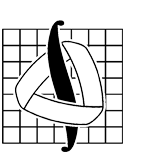
\includegraphics[width=20mm]{pics/mmlogo.png}}%
  \end{center}
\end{figure}
\vspace{4cm}
\Large{
ЗАДАЧИ ФИЗИКО-МЕХАНИЧЕСКОГО ПРАКТИКУМА ПО ГАЗОВОЙ И ВОЛНОВОЙ ДИНАМИКЕ
}\\
\vspace{4cm}
\end{center}
\end{titlepage}

\tableofcontents

\anonsection{Раздел 1}
\anonsubsection{Задача 1. Продольное соударение упругих стержней}
\anonsubsection{Задача 2. Сверхзвуковое обтекание клина}
\anonsubsection{Задача 3. Поперечные колебания бруса}
\anonsubsection{Задача 4. Распространение и отражение гидравлического прыжка}
\anonsection{Раздел 2}
\anonsubsection{Задача 1. Волны разгрузки в гибких растяжимых нитях}
\anonsubsection{Задача 2. Изучение процесса разгона поршня в стволе пневматической установки}
\anonsubsection{Задача 3. Нелинейные волны сжатия (растяжения) сдвига в тонкостенной цилиндрической трубе}
\anonsubsection{Задача 4. Прямой экспериментальный метод построения ударных диаграмм сжатия грунтов}
\anonsubsection{Задача 5. Сверхзвуковое обтекание кругового конуса}
\anonsubsection{Задача 6. Соударение двух упругих тел}
\anonsubsection{Задача 7. Экспериментальное исследование подводного взрыва сферического заряда}
\anonsubsection{Задача 8. Влияние вращения цилиндра, находящегося в поперечном потоке, на распределение давления по его поверхности}


\end{document}
